\section{Case Studies}\label{sec:case_study}

\subsection{Unitrans}

UC Davis operates a bus network connecting the UC Davis campus to locations around the City of Davis called Unitrans. During academic sessions, this service operates 18 regular routes. The routes are each referred to by a letter. All buses are serviced from a single depot located on nearby the two terminal stations. On a given week the Monday service contains 2,263 individual trips (after merging out and in legs). Start times for the trips are shown in Figure \ref{fig:unitrans_trips}.

\begin{figure}[H]
	\centering
	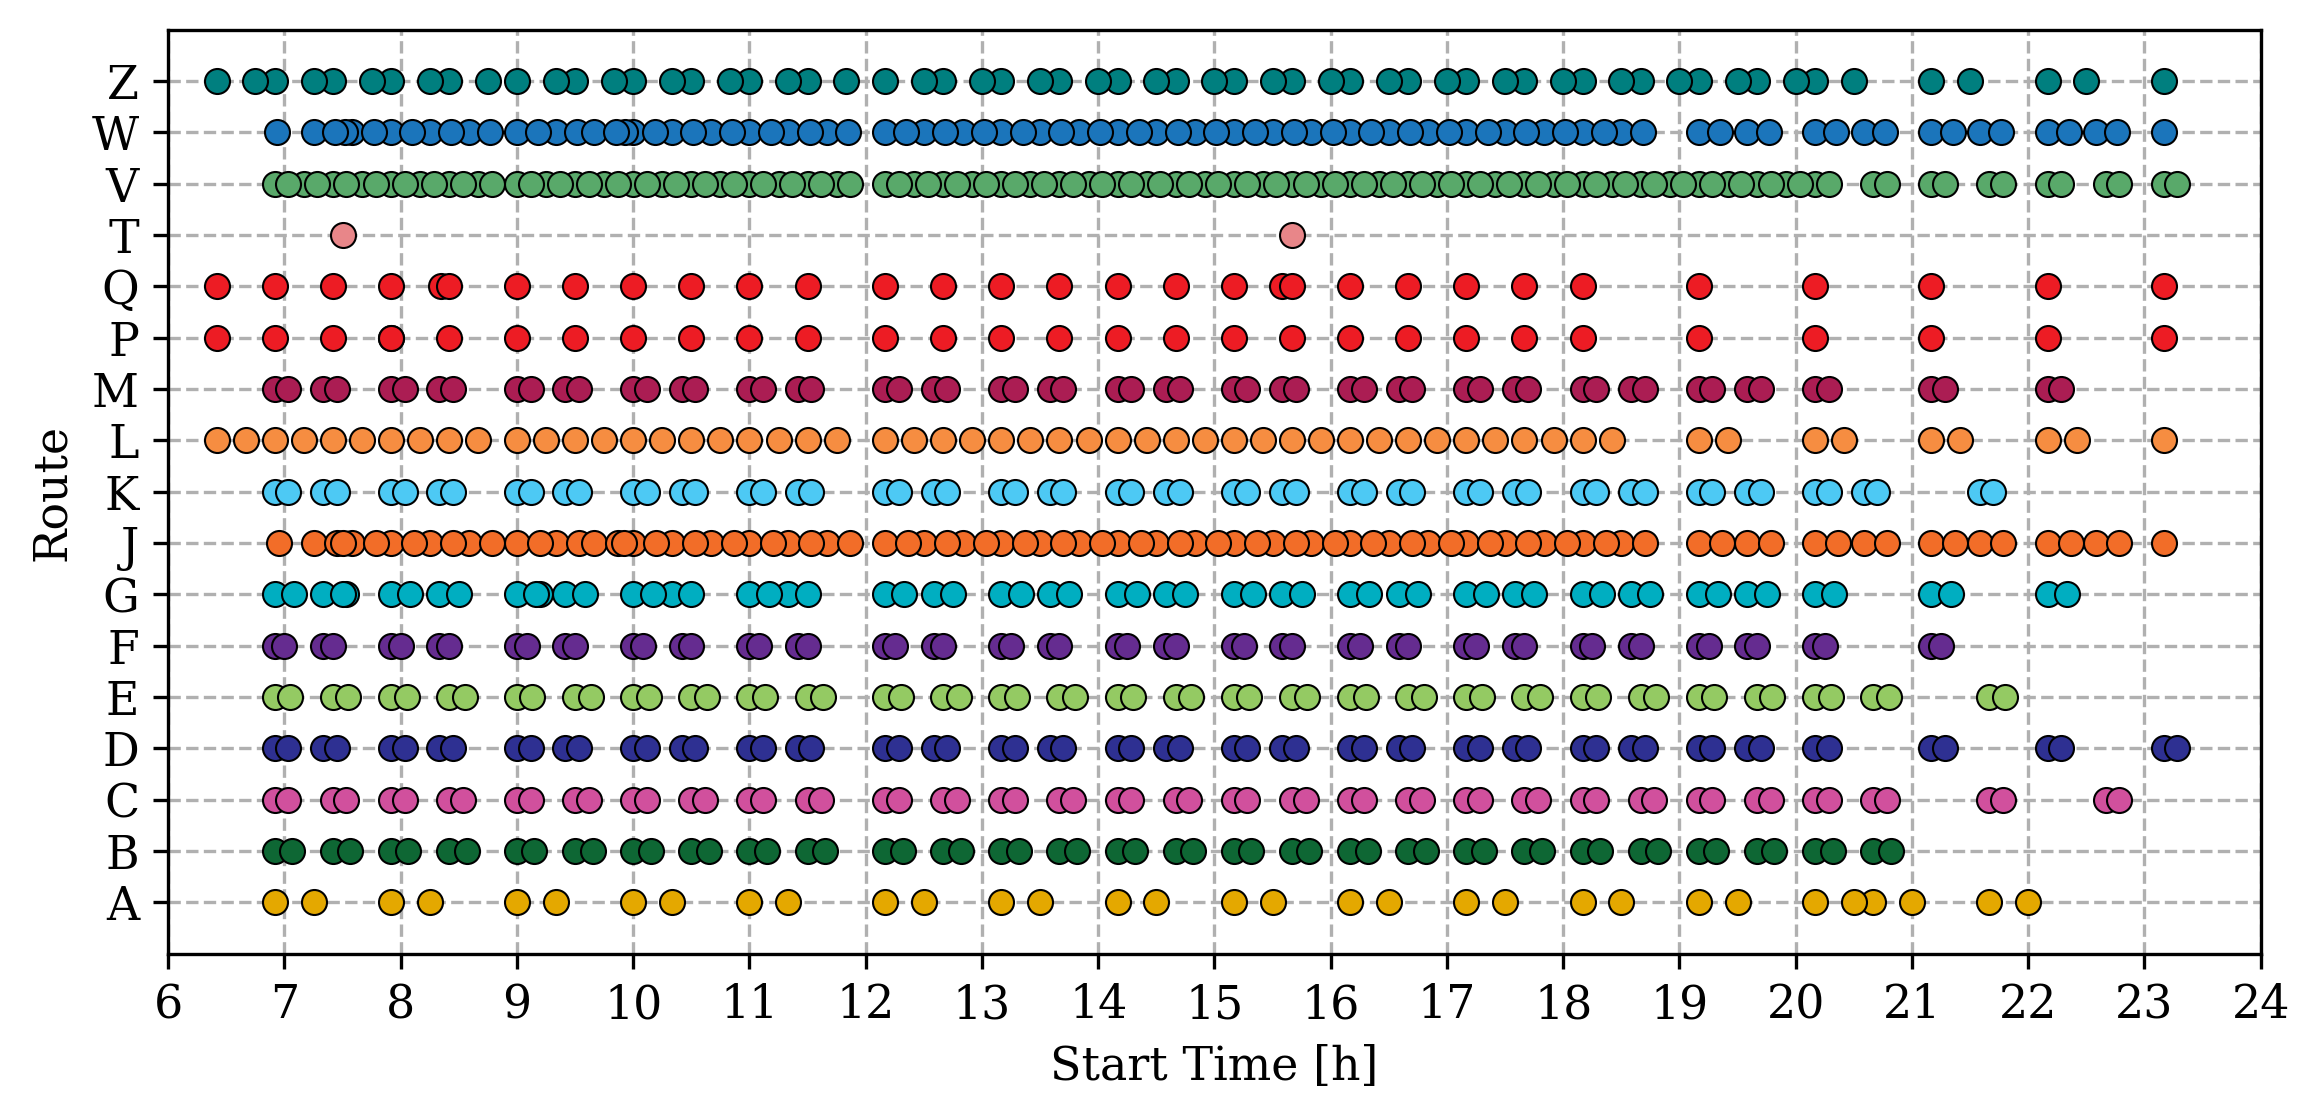
\includegraphics[width = \figurewidth]{figs/unitrans_trips.png}
	\caption{}
	\label{fig:unitrans_trips}
\end{figure}

The vehicle and supply equipment models used in this case study are inexact and meant to be representative rather than specific. Actual costs will vary meaningfully by operator. Parameters given are informed by technical reports of real world implementations \cite{Jeffers_2021_OSTI, Eudy_2021_OSTI, Post_2023_OSTI} and journal papers \cite{Rout_2022_H, Chen_2024_S, Sistig_2025_SMT}.

For these examples five different vehicle types are considered. These include three different \glspl{ev}, a \gls{srbev}, \gls{mrbev}, and a \gls{lrbev}, a \gls{fcev}, and a diesel \gls{icev}. The bus models are described in Table \ref{tab:vehicle_types}. The technical parameters are based on NewFlyer models \cite{CHVIP_2025} and the costs are based on APTA purchase prices data \cite{APTA_2025}.

\begin{table}[H]
	\centering
	\caption{}
	\label{tab:vehicle_types}
	\begin{tabular}{|C{.2\linewidth}|C{.2\linewidth}|C{.2\linewidth}|C{.2\linewidth}|C{.2\linewidth}|}
		\hline Vehicle Type & Capacity [kWh] & Maximum Supply Rate [kW] & Consumption [kWh / km] & Unit Cost [USD] \\
		\hline \gls{srbev} & 440 & 350 & 1.25 & 800,000 \\
		\hline \gls{mrbev} & 550 & 350 & 1.3 & 1,000,000 \\
		\hline \gls{lrbev} & 660 & 350 & 1.35 & 1,200,000 \\
		\hline \gls{fcev} & 1,277.5 & 10,950 & 2.81 & 1,600,000 \\
		\hline \gls{icev} & 5,180 & 88,800 & 2.23 & 280,000 \\
		\hline
	\end{tabular}
\end{table}

The four different supply port types in Table \ref{tab:port_types} are also considered. These are AC chargers, DC chargers, Liquefied Hydrogen pumps, and Diesel pumps. The technical and cost parameters are based on transit operator reports. Emissions values are taken from US EPA equivalencies. Electric emissions use the California power grid intensity. H2 production and liquefaction are assumed to be grid powered and thus the emissions intensity is that of the California power grid multiplied by a constant reflecting the energy overhead required. Although the difference in emissions intensity appears small between the energy types, actual emissions scale with energy used and the \glspl{ev} have much lower energy consumption values leading to much lower gross emissions per km driven.

\begin{table}[H]
\centering
\caption{}
\label{tab:port_types}
\begin{tabular}{|C{.2\linewidth}|C{.2\linewidth}|C{.2\linewidth}|C{.2\linewidth}|C{.2\linewidth}|}
	\hline port Type & Maximum Supply Rate [kW] & Emissions [gC02 / kWh] & Unit Cost [USD] & Fixed Cost [USD]\\
	\hline AC-PLUG & 19 & 225.6 & 5,000 & 10,000\\
	\hline DC-PLUG & 150 & 225.6 & 30,000 & 50,000 \\
	\hline LH2-PUMP & 10,950 & 322.3 &  100,000 & 250,000 \\
	\hline DIESEL-PUMP & 88,800 & 275.1 & 30,000 & 50,000 \\
	\hline
\end{tabular}
\end{table}

The single depot that Unitrans operates out of is space limited both in terms of overall parking and in terms port capacity. In this example the parking spaces for the fleet are limited to 60 which also limits the fleet size to 60 buses. There are 10 total available spaces for dedicated charging/fueling. This limits the total number of DC charging stations, hydrogen pumps, and diesel pumps to 10. Because AC chargers are small in footprint one can be added for each parking spot.

In this example the objectives are capital cost and daily cost. Capital Cost includes the costs of purchasing vehicles and supply equipment. Vehicle cost is based only on unit cost while supply equipment cost includes both the unit cost per port and a fixed cost paid before any ports of a given type can be installed. Daily cost encompasses operational costs, energy costs, and labor costs. Operational costs are assumed to scale with distance driven, energy costs are assumed to scale with energy consumed, and labor costs are assumed to scale with operating time (a fixed hourly rate of 20 USD per hour is used for drivers).

Given the vehicle and port options and the weekday schedule, an optimization was run with the following hyper-parameters: population size $M = 150$, generations range $N^- = 300$, $N^+ = 500$, probability of crossover $\phi_c = 0.5$, and probability of mutation $\phi_m = 0.05$. Iteration was terminated after 344 generations when zero children were selected for 5 consecutive generations. The evolution of the population over time is displayed in Figure \ref{fig:evolution_unitrans}.

\begin{figure}[H]
	\centering
	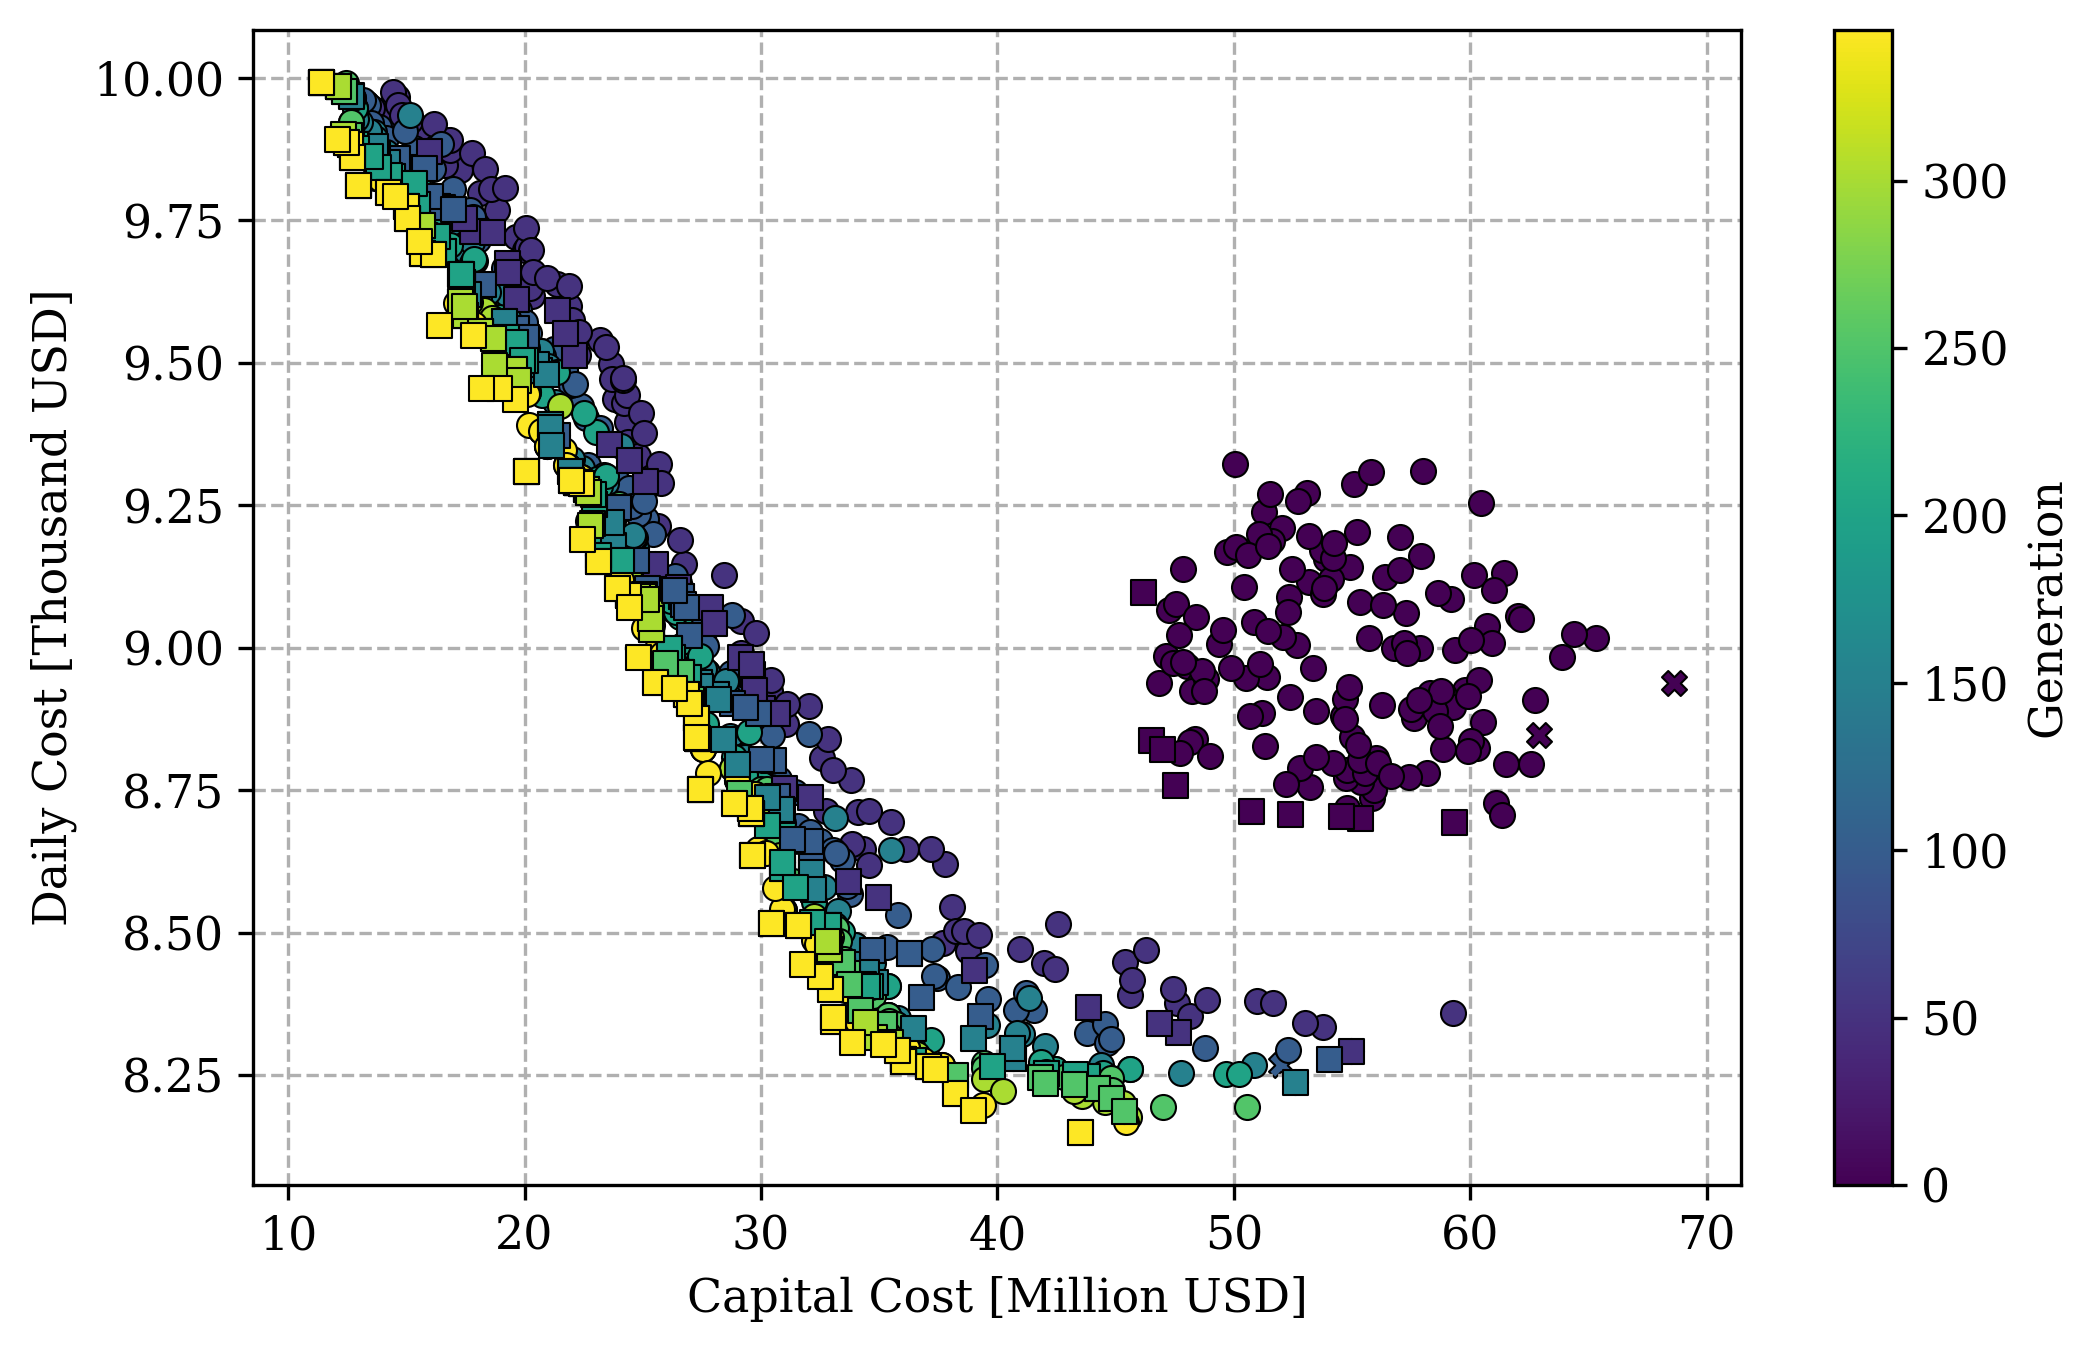
\includegraphics[width = \linewidth]{figs/evolution_unitrans.png}
	\caption{}
	\label{fig:evolution_unitrans}
\end{figure}

As can be seen, the pace of evolution is rapid initially but becomes slow after about 100 iterations. Possibly, different hyper-parameter settings could result in quicker convergence at the cost of increasing the likelihood if premature termination. The final Pareto front and fleet compositions and sizes are shown in Figures \ref{fig:unitrans_baseline_scatter_pie} and \ref{fig:unitrans_baseline_stacked_bar}.

\begin{figure}[H]
	\centering
	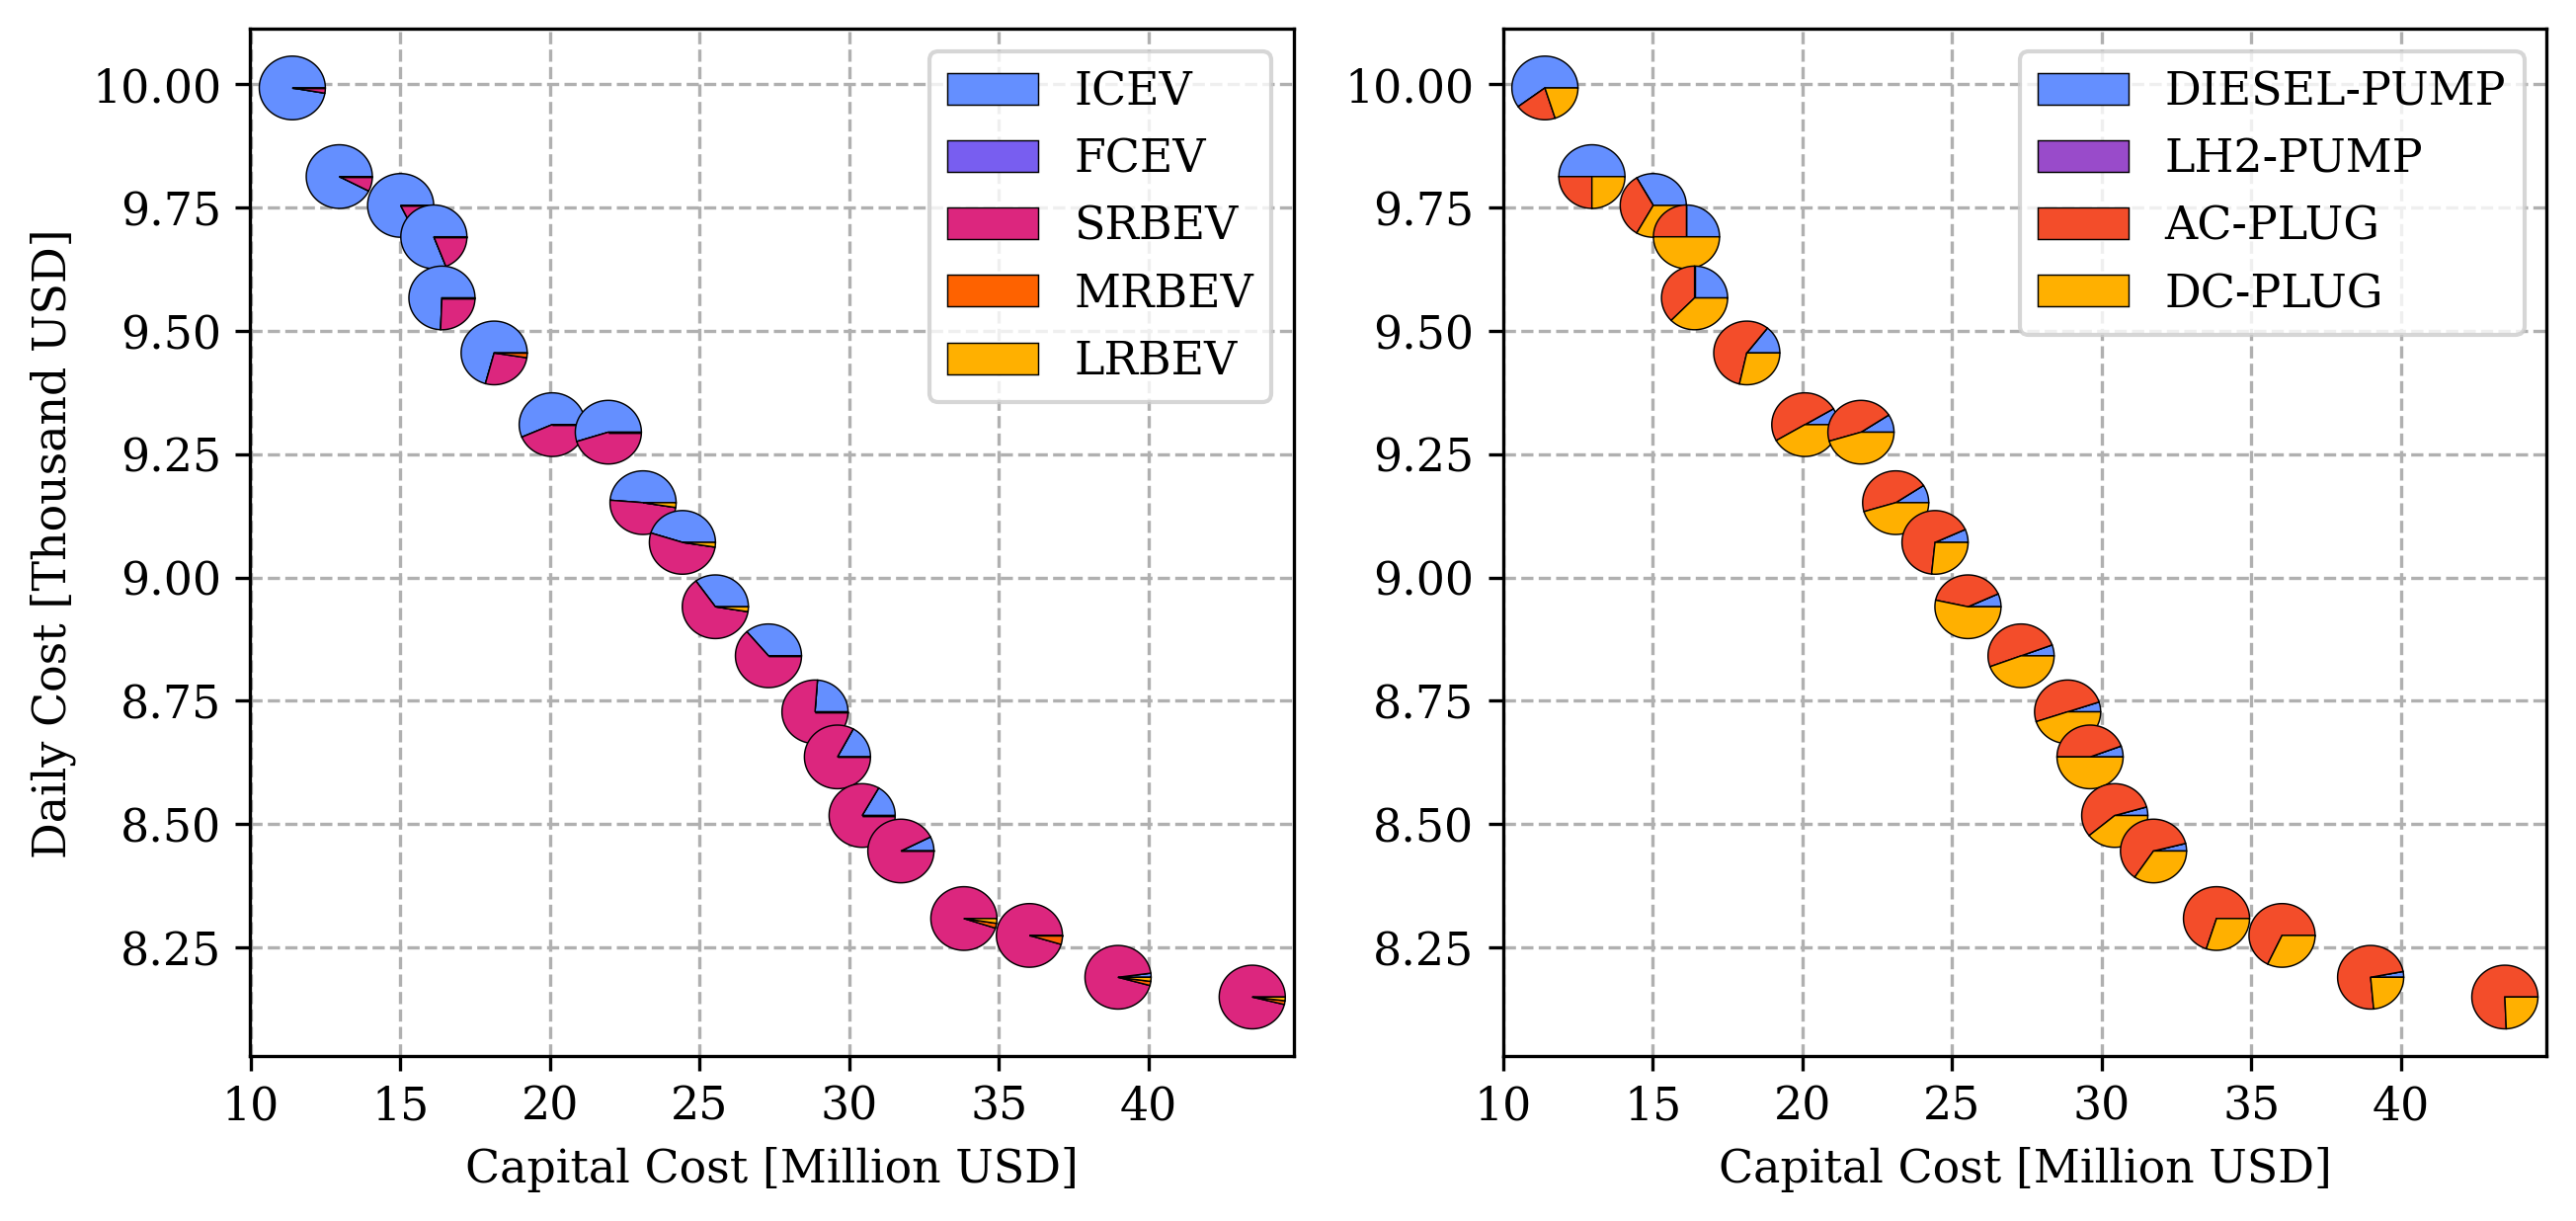
\includegraphics[width = \linewidth]{figs/unitrans_baseline_scatter_pie.png}
	\caption{}
	\label{fig:unitrans_baseline_scatter_pie}
\end{figure}

\begin{figure}[H]
	\centering
	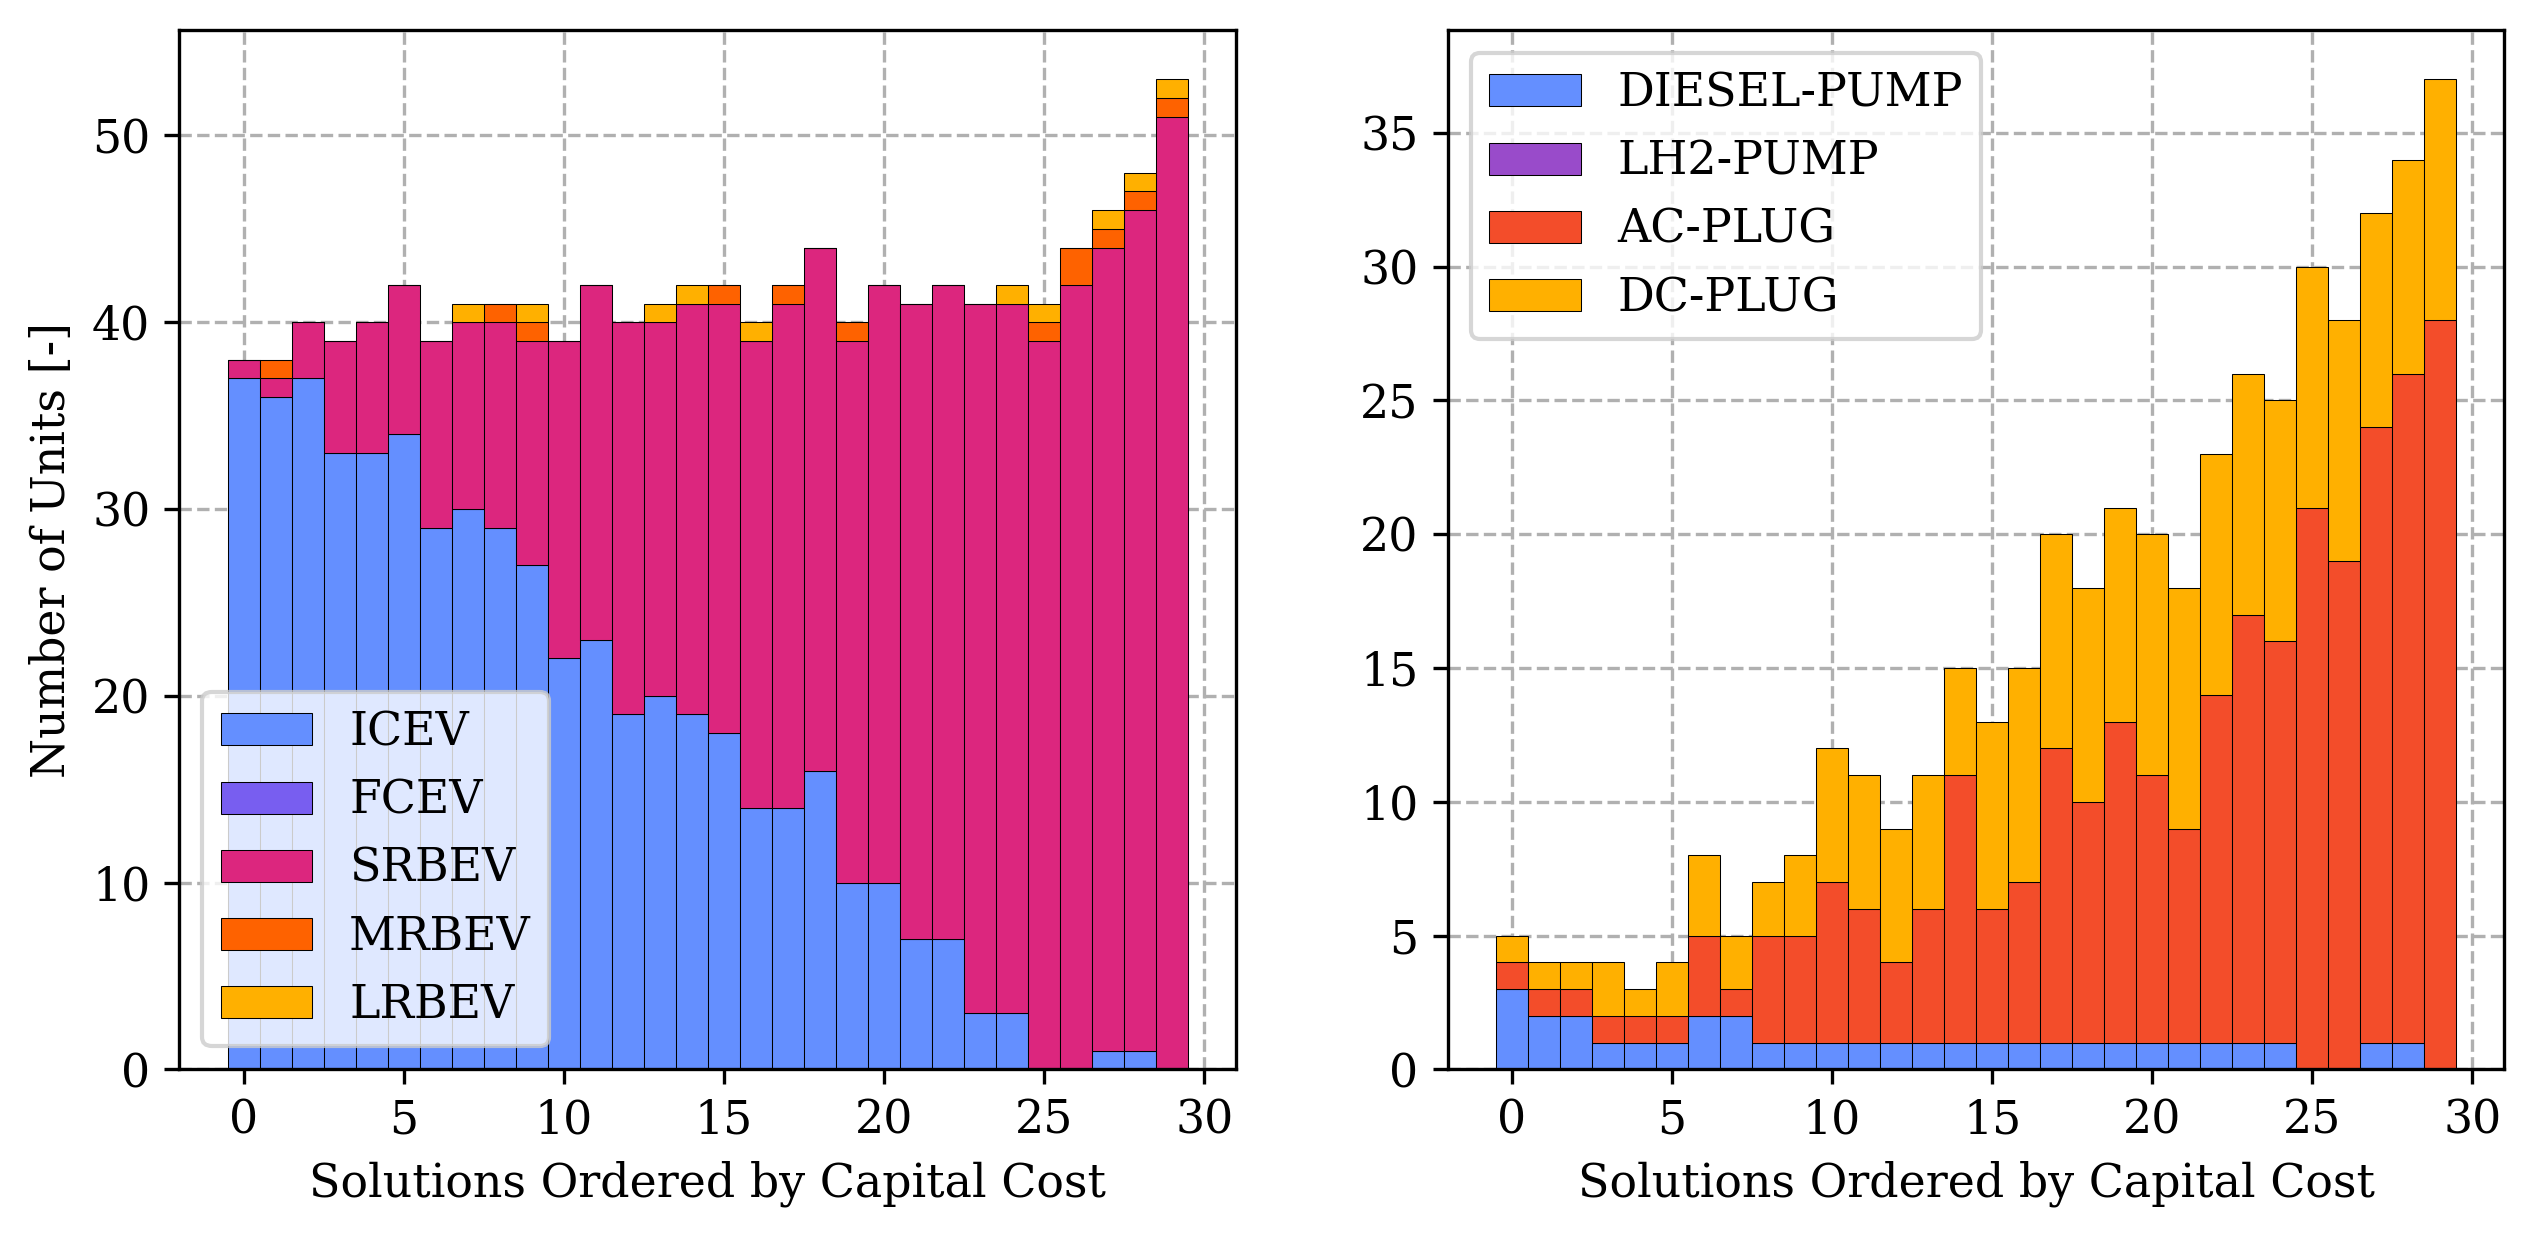
\includegraphics[width = \linewidth]{figs/unitrans_baseline_stacked_bar.png}
	\caption{}
	\label{fig:unitrans_baseline_stacked_bar}
\end{figure}

Figure \ref{fig:unitrans_baseline_scatter_pie} shows the Pareto front as a scatter plot of pie charts for both vehicles and supply infrastructure. The composition of the fleet is reflected in the slices of the pie charts. As can be seen, solutions which present low capital costs and high daily costs are dominantly composed of Diesel \glspl{icev}. On the opposite end high capital cost, low daily cost solutions are dominantly composed of \glspl{srbev}. Options such as the \gls{mrbev}, \gls{lrbev}, and \gls{fcev} are minimally present. This is likely due to the small geographic area Unitrans services and the frequency of trips. Because the vehicle fleets at the high daily cost end of the front are \gls{icev} dominated, there is little reason to build other infrastructure. Additionally because \gls{icev} fueling is rapid, there is no reason to build a large number of pumps. Moving towards the high capital cost end of the front, \gls{bev} charging infrastructure becomes more prevalent. Initially this is largely DC chargers due and eventually becomes mostly AC chargers due to the constraint on the number of DC chargers that can be built. Vehicle fleet sizes remain roughly constant at around 40 vehicles throughout the front until the high-capita-cost extreme. The actual Unitrans fleet contains around 50 vehicles but this number accounts for maintenance cycles which are not modeled in this paper.

\subsection{SFMTA}

The second case study concerns a much larger bus network. \gls{sfmta} operates a bus network which connects locations within the city of San Francisco which is geographically large and densely populated by US standards. A Monday schedule for \gls{sfmta} consists of 8,993 scheduled trips operating from six primary depots. Unlike Unitrans, route terminals are scattered throughout the city. Weekday service runs from 4 AM through midnight and most routes are serviced with high frequency as seen in Figure \ref{fig:sfmta_trips}.

\begin{figure}[H]
	\centering
	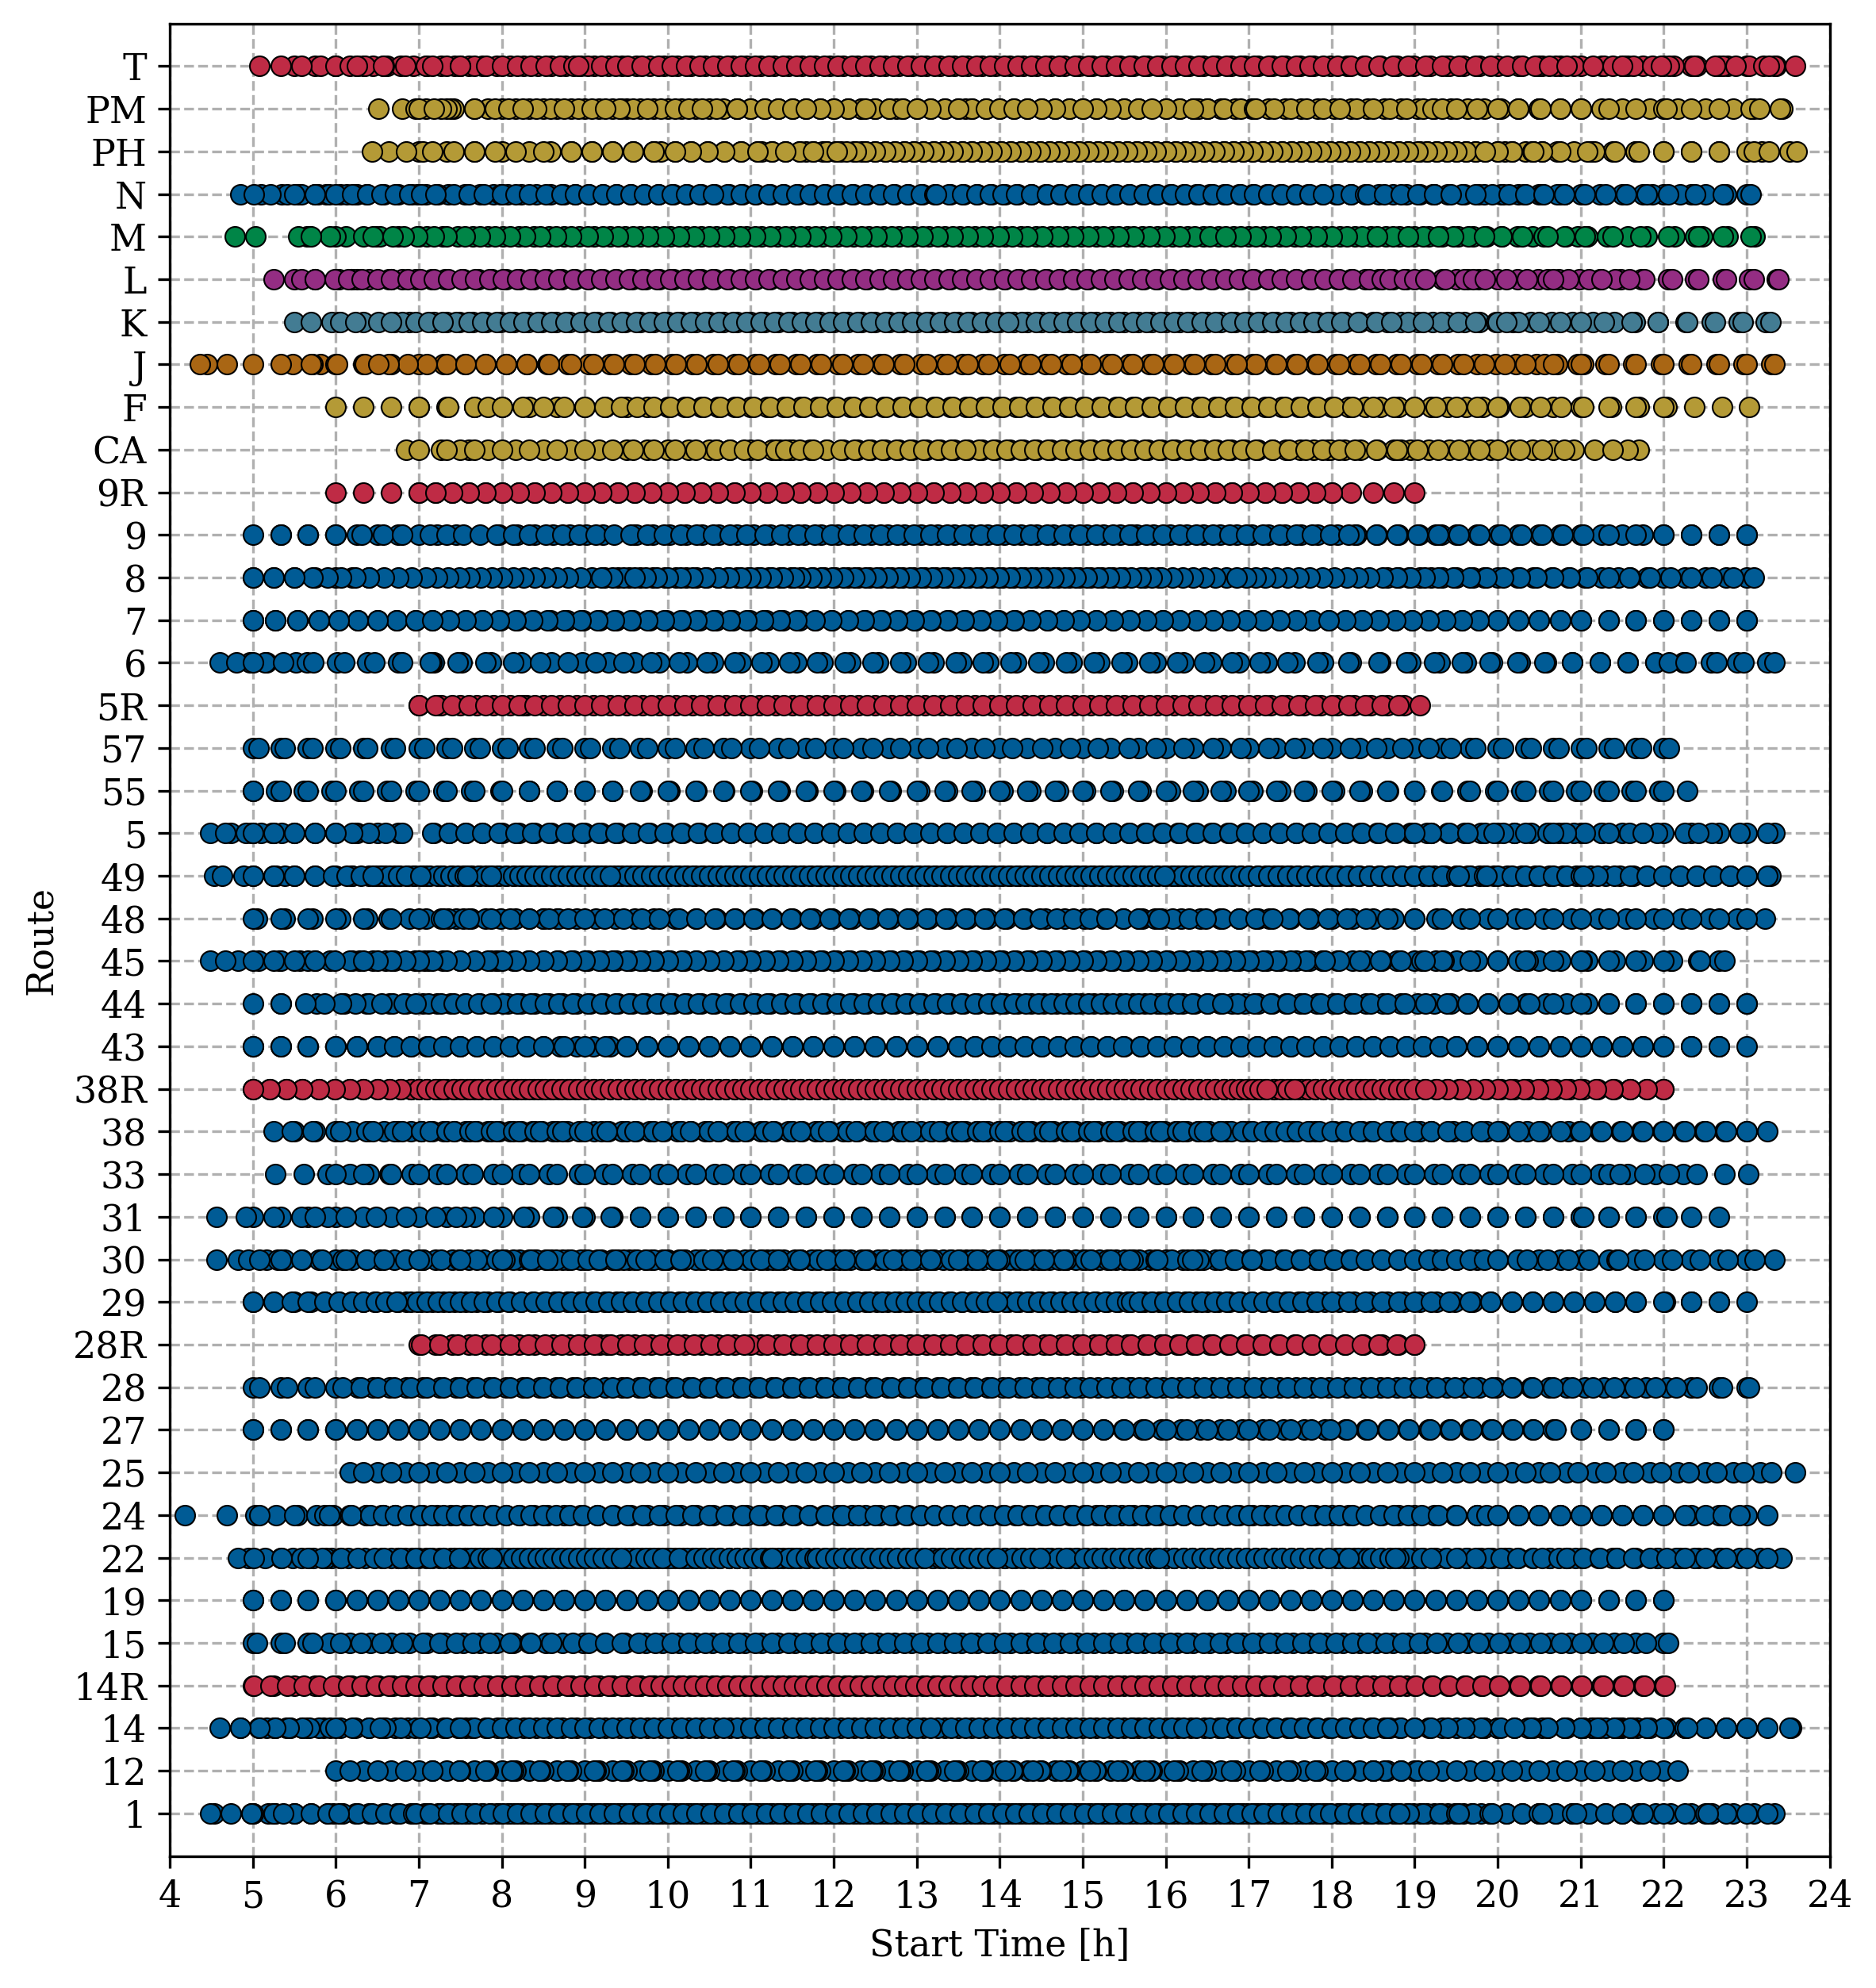
\includegraphics[width = \figurewidth]{figs/sfmta_trips.png}
	\caption{}
	\label{fig:sfmta_trips}
\end{figure}

Using the same vehicle and port options as with Unitrans, an optimization was run with the following hyper-parameters: population size $M = 200$, generations range $N^- = 500$, $N^+ = 1000$, probability of crossover $\phi_c = 0.5$, and probability of mutation $\phi_m = 0.15$. Iteration was terminated after 759 generations when zero children were selected for 5 consecutive generations. The evolution of the population over time is displayed in Figure \ref{fig:evolution_sfmta}.

\begin{figure}[H]
	\centering
	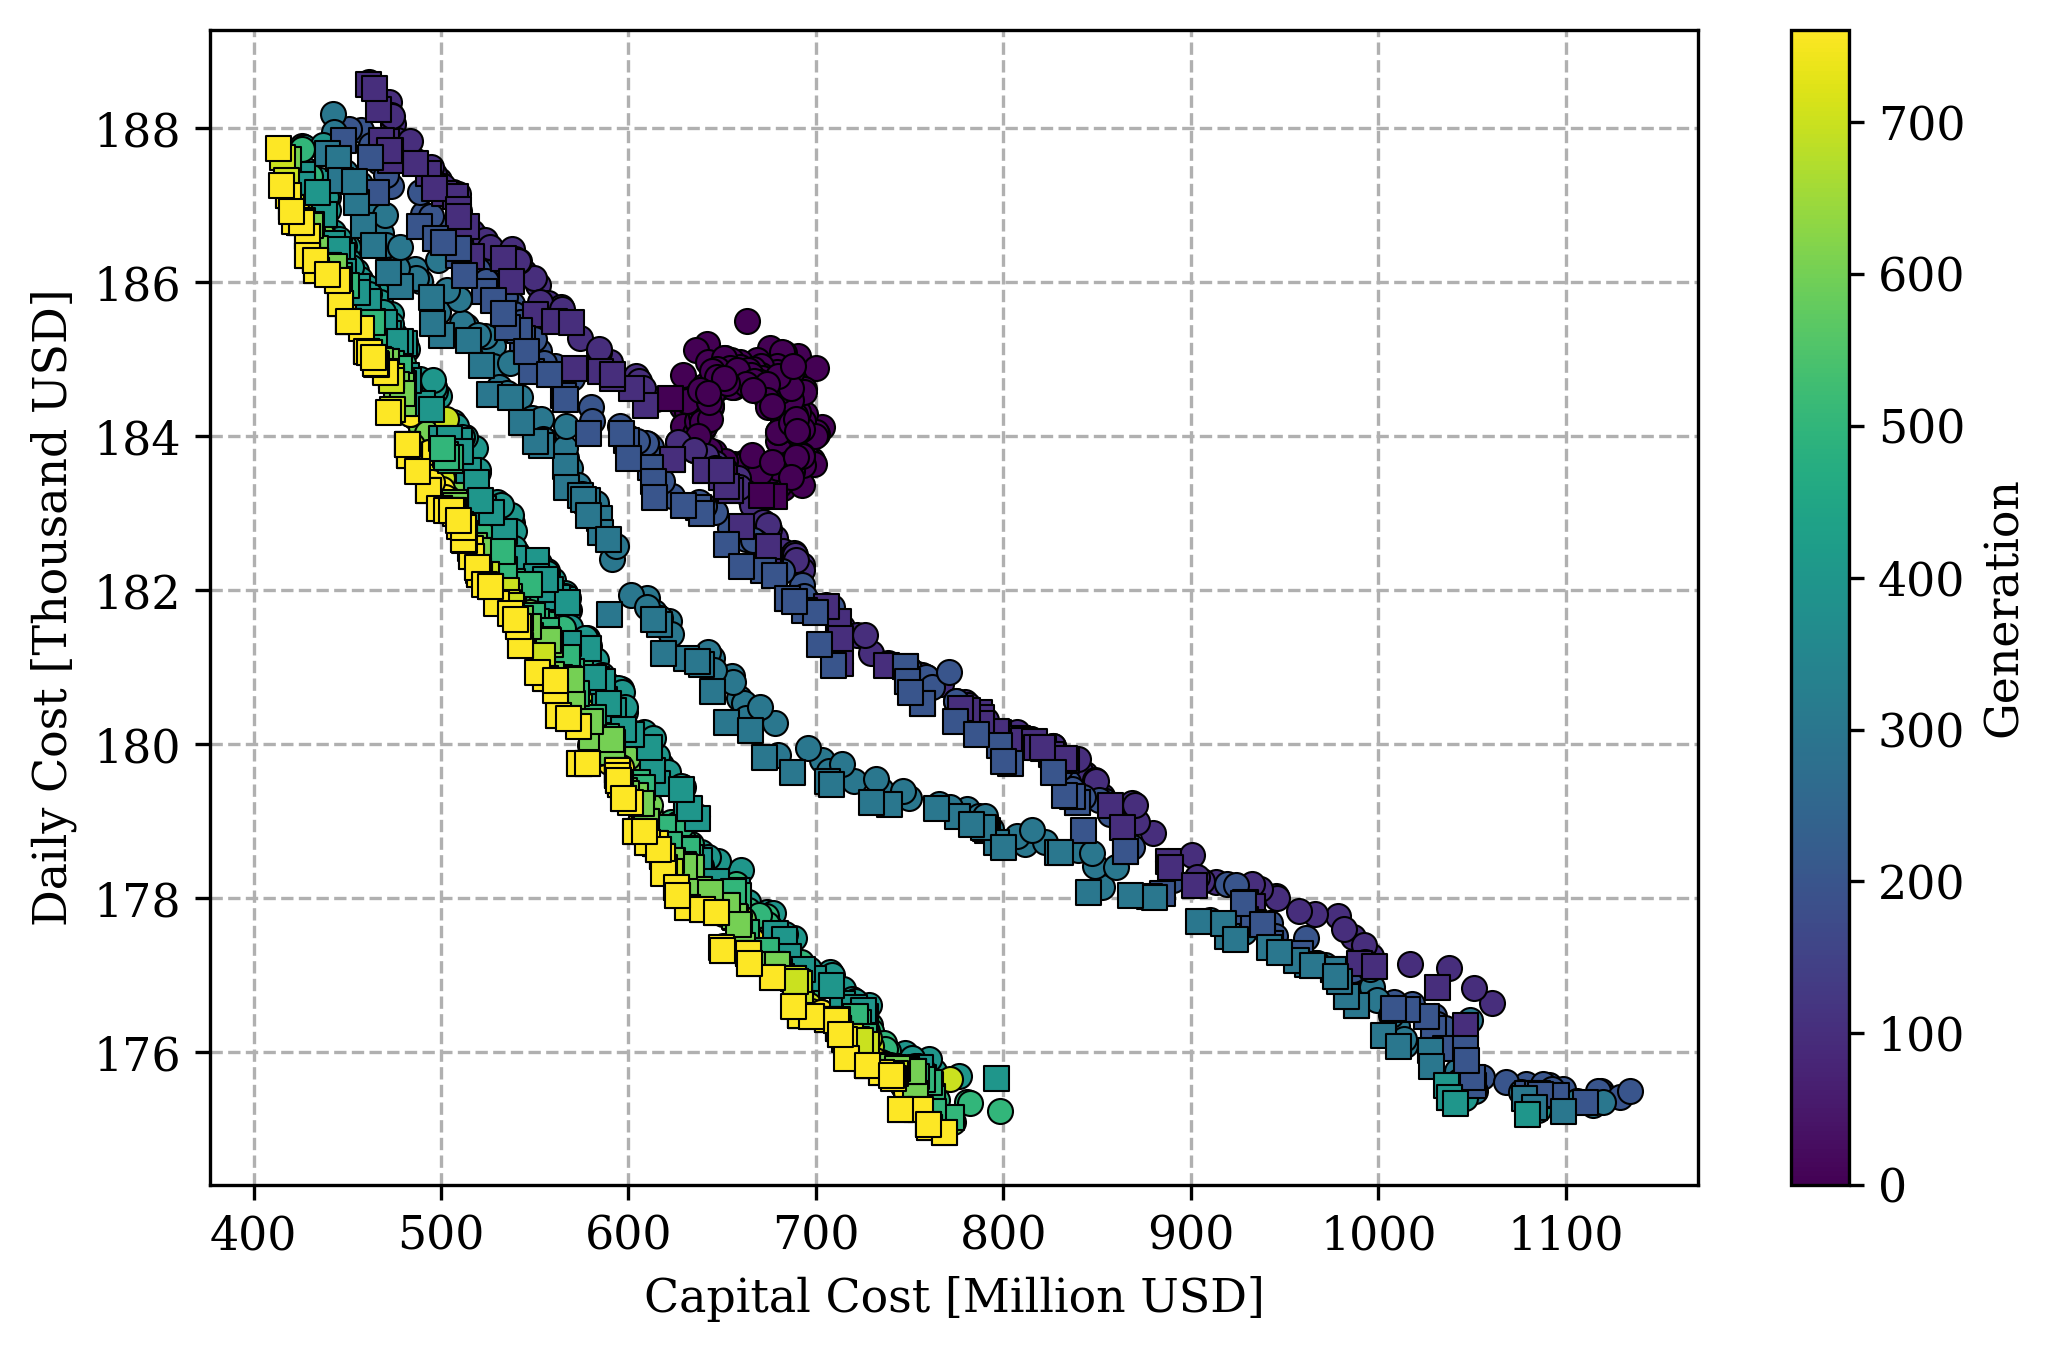
\includegraphics[width = \linewidth]{figs/evolution_sfmta.png}
	\caption{}
	\label{fig:evolution_sfmta}
\end{figure}

Being a much larger network with a exponentially  greater number of possible configurations, the \gls{sfmta} optimization converged slower. Where the Pareto front reached its approximate final shape within 100 generations for Unitrans, this took around 400 generations for \gls{sfmta}. For the \gls{sfmta} case study, a higher mutation probability was used in order to more efficiently explore the design space at the cost of additional randomness. After reaching an approximate final shape, several hundred generations were required before reaching convergence.

The Pareto front for \gls{sfmta} shows a similar but meaningfully different trade-off to that found for Unitrans reflecting differences in routes, schedules, and economies of scale. As seen in Figure \ref{fig:scatter_pie_vehicles_baseline_sfmta}, the Pareto front for \gls{sfmta} contains substantially mixed fleets with non-negligible numbers of \glspl{mrbev} and \glspl{lrbev} alongside the dominant \glspl{icev} and \glspl{srbev}. On the other hand, supply infrastructure is much more uniform in the \gls{sfmta} Pareto front with AC charging dominating DC charging as seen in Figures \ref{fig:scatter_pie_baseline_sfmta} and \ref{fig:stacked_bar_baseline_sfmta}. This is in contrast in the Unitrans Pareto front which contains substantially DC based solutions. The most important differences are the scale of the bus fleets with additional bus purchases playing a smaller role in overall capital budget for \gls{sfmta} than for Unitrans, the time and energy required to travel from route terminals to depots to charge, and lack of depot supply infrastructure constraints. Unitrans operates over a substantially smaller geographic area and all routes terminate close to the depot allowing for buses to easily return to depot to top-up during the day. This strategy is not as viable for \gls{sfmta}.

\begin{figure}[H]
	\centering
	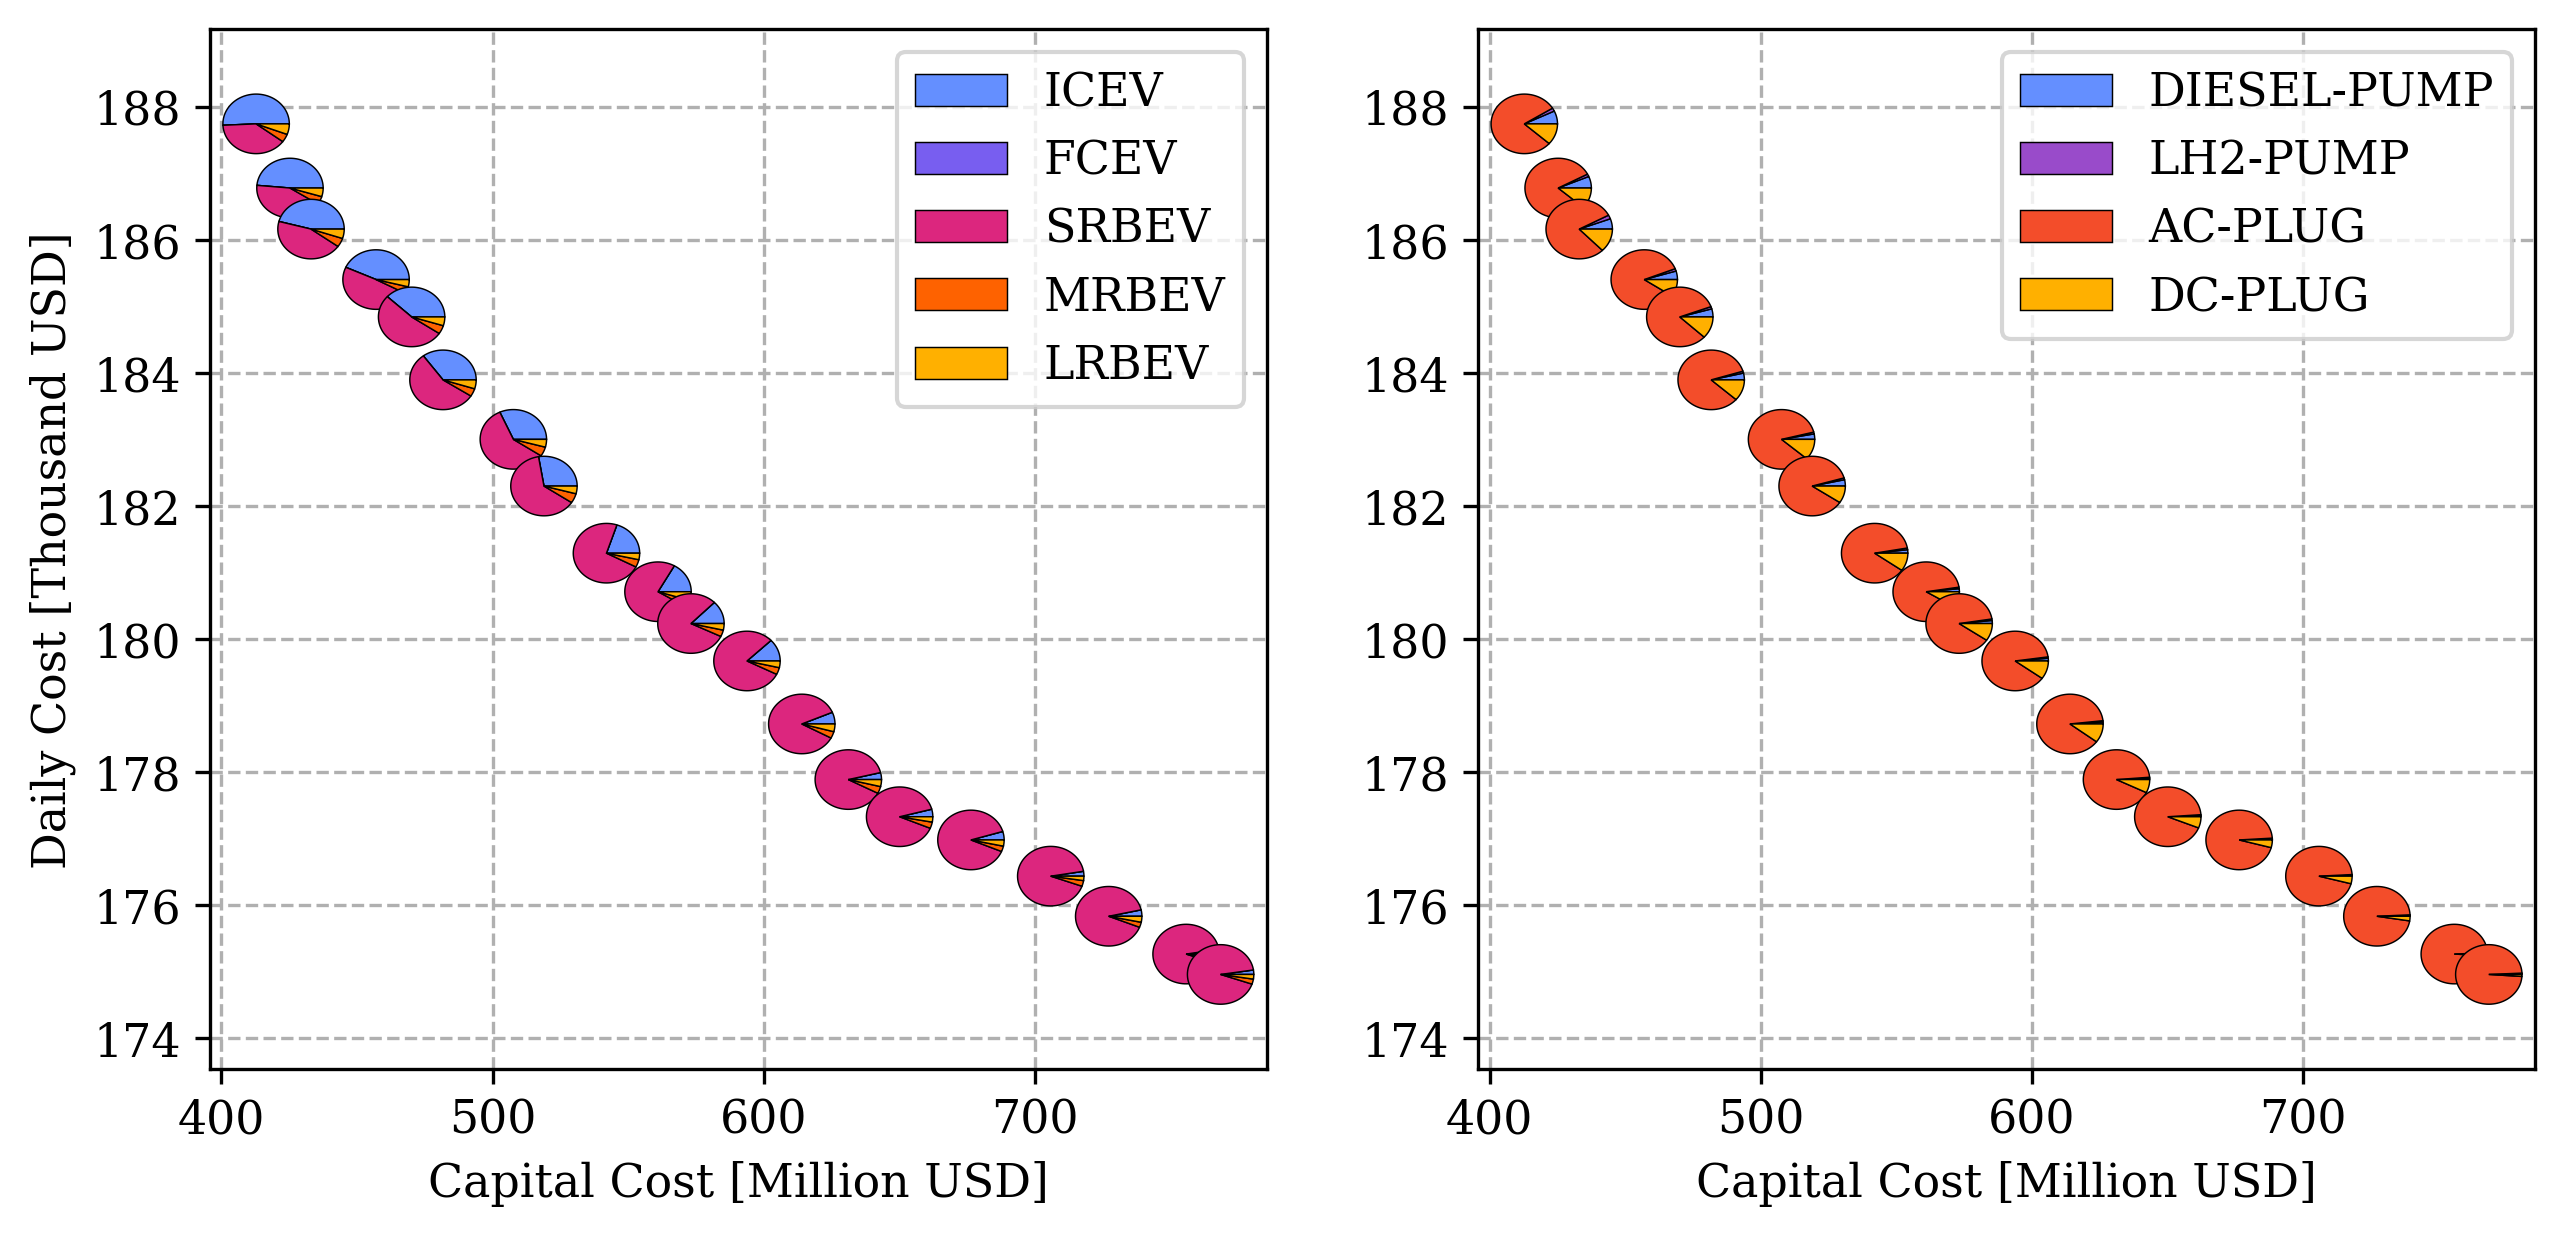
\includegraphics[width = \linewidth]{figs/sfmta_baseline_scatter_pie.png}
	\caption{}
	\label{fig:scatter_pie_baseline_sfmta}
\end{figure}

\begin{figure}[H]
	\centering
	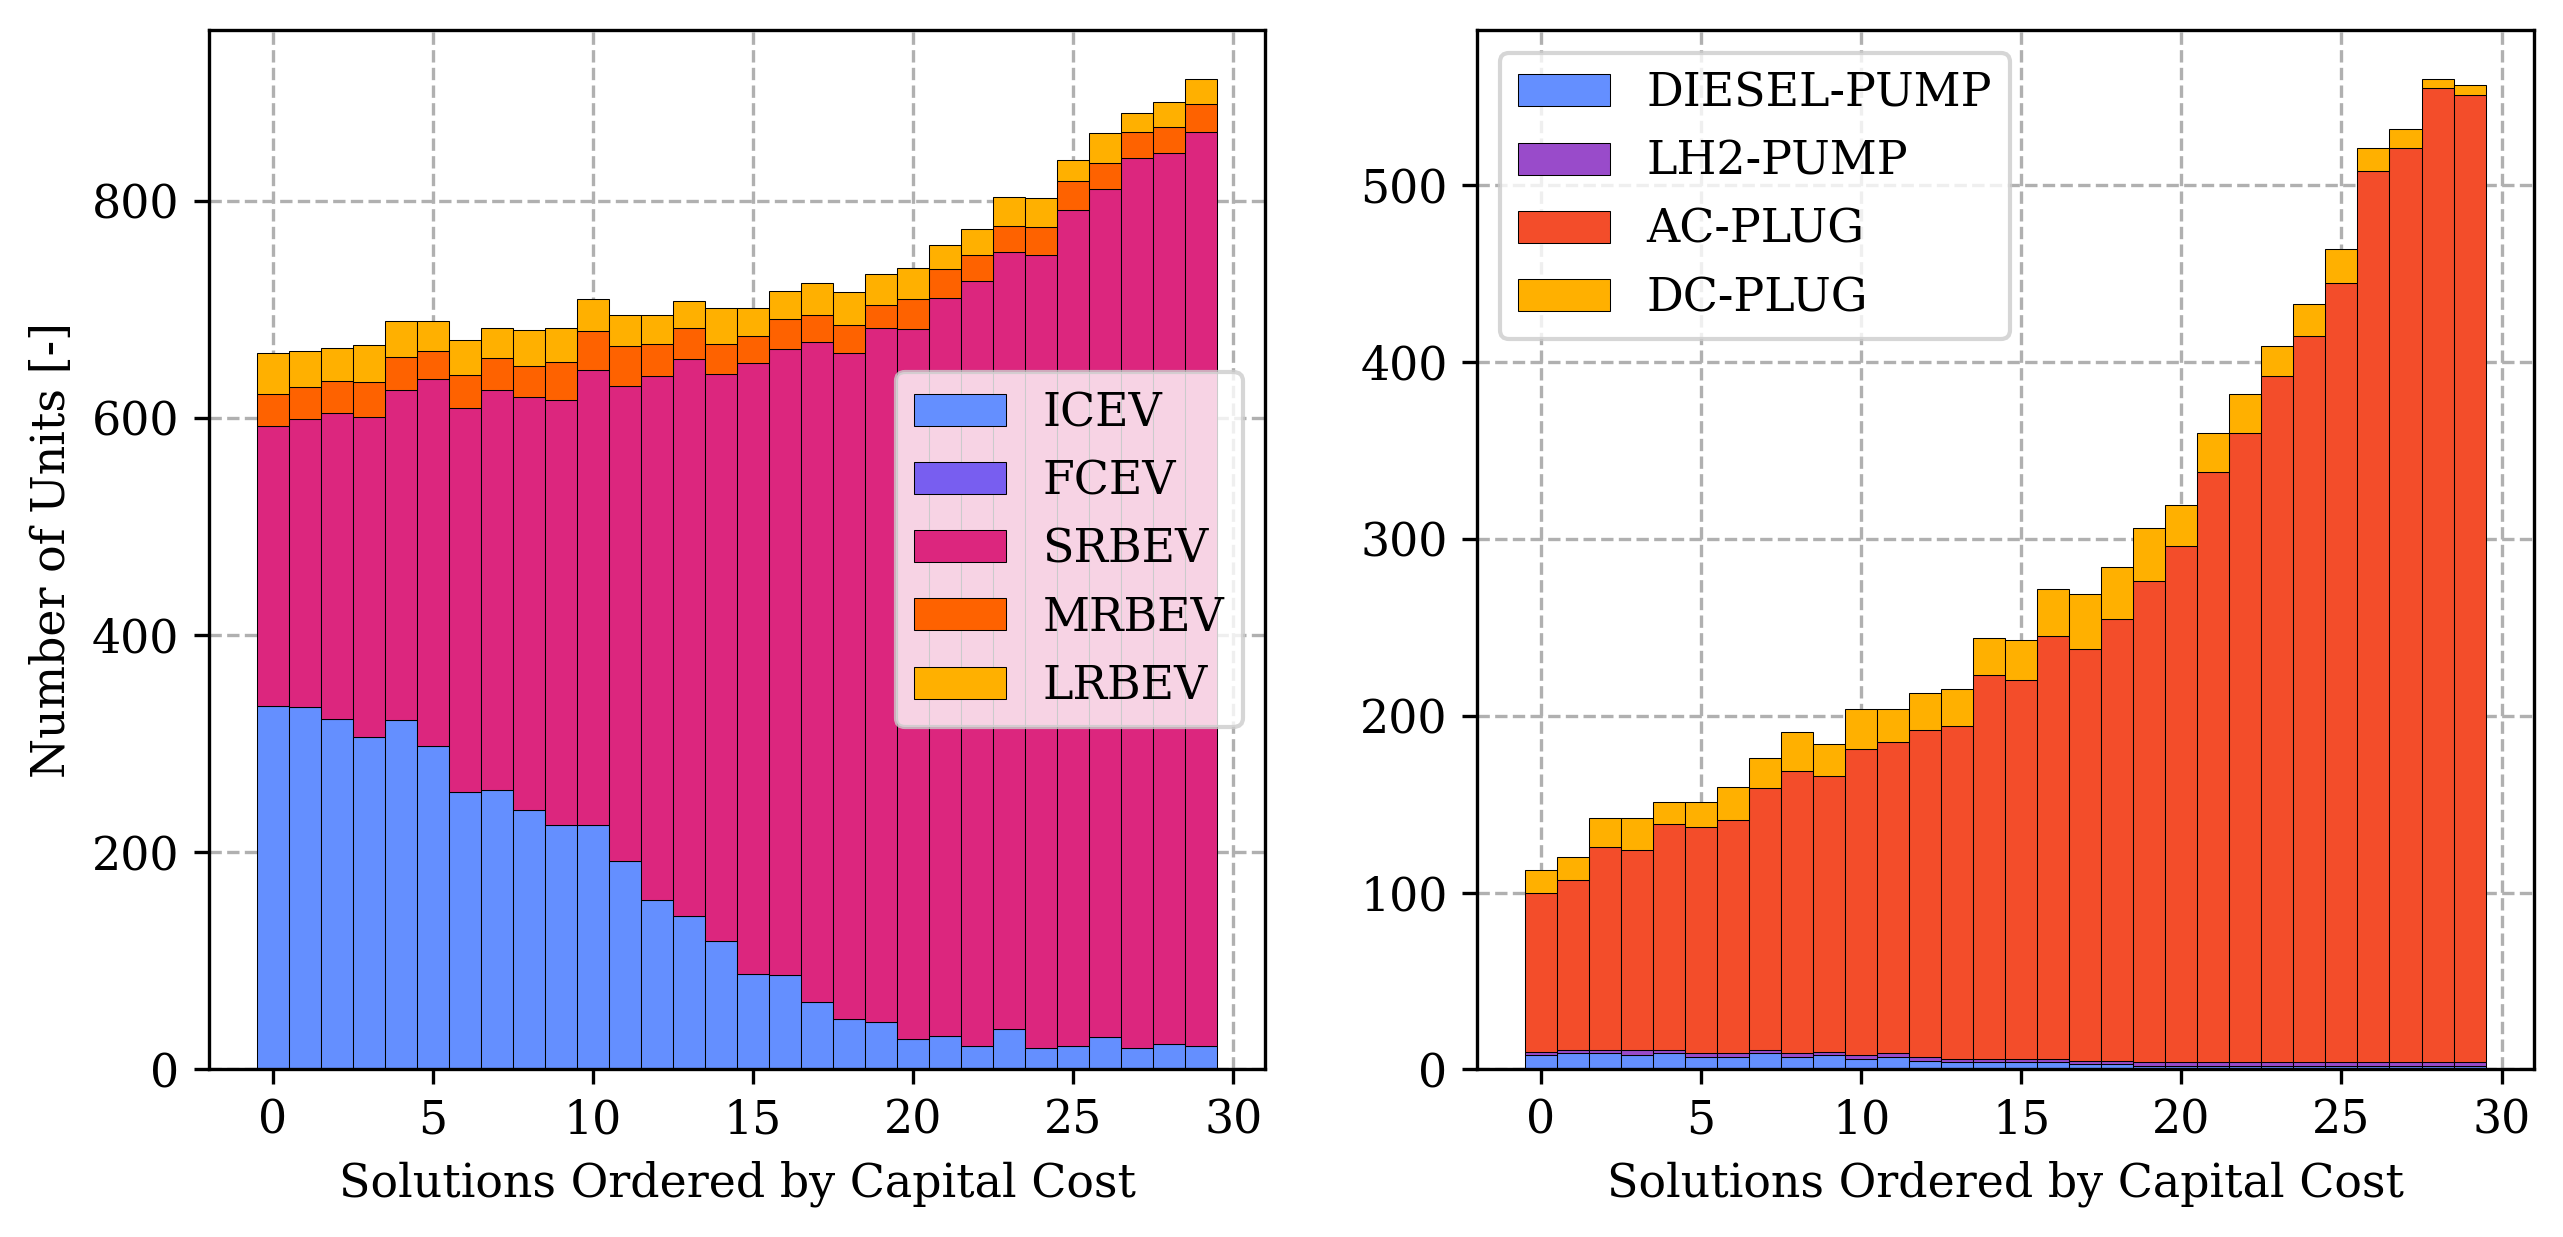
\includegraphics[width = \linewidth]{figs/sfmta_baseline_stacked_bar.png}
	\caption{}
	\label{fig:stacked_bar_baseline_sfmta}
\end{figure}

The actual size of the SFMTA bus fleet is around 850 buses. The solutions produced are in line with this number allowing for the lack of maintenance schedules in the model. The case studies shown here serve to show that the method produces a realistic Pareto front for realistically-scaled networks. The examples used are simplistic in representation of the network (for example neither elevation nor catenary charging were considered), representation of costs, and representation of constraints. All data used in case-study construction is public domain data. The results presented should not be treated as exemplary rather than accurate. Stakeholders applying the method will have much more detailed inputs and, as a result, can obtain accurate solutions. With this information, decision makers can determine what type of fleet to acquire depending on their relative sensitivity to various cost categories. Neither equipment models nor cost functions are integral to the method. More sophisticated and altogether different cost functions and models can be used without changing the core of the method and without changing computational complexity.